\begin{homeworkProblem}

\textbf{Chicken-Egg with Unknown Parameters:} The parameter setting: $\lambda=10, a=b=1, x=7$.

(a) Implement a Gibbs sampler to find the posterior mean and the variance of $p$ after observing $x$ hatched eggs.

(b) Implement a Metropolis-Hastings algorithm to find the posterior mean and variance of $p$ after observing $x$ hatched eggs.

(c) Compare such two methods of MCMC.

\solution

Let $N\sim\Pois(\lambda)$ donates number of eggs. \\
The prior distribution of the hatch probability is $P\sim\Beta(a,b)$. \\
$X|P=p\sim\Pois(\lambda p)$ is the number of hatched eggs, $N-X|P=p\sim\Pois(\lambda(1-p))$ is the number of unhatched eggs.

(a) Directly sample the conditional probability above is complex, so we consider the conditional joint distribution of $X,N|P$: \\
Since $X|N=n,P=p\sim\Bin(n,p)$, and we have the prior $P\sim\Beta(a,b)$, from the Beta-Binomial conjugate, we can get that
$$P|N=n,X=x\sim\Beta(a+x,b+n-x)$$
And from the definition of $N$ and $X$, we have
$$f_{N|P,X}(n|P=p,X=x) \sim x + \Pois(\lambda(1-p))$$
The conditional distributions are all easy to sample, so we can use the Gibbs sampling to sample the joint distribution of $P,N|X$, then the marginal distribution of $P|X=x$ and $N|X=x$ can be calculated. Set the initial state to be $p_0=0.5, n_0=7$.  The sampling results are as follows:
\begin{figure}[h]
    \centering
    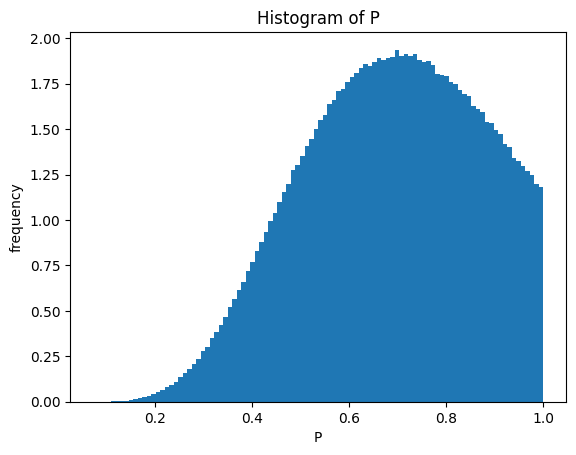
\includegraphics[width=0.49\textwidth]{./figure/p8/Gibbs_P.png}
    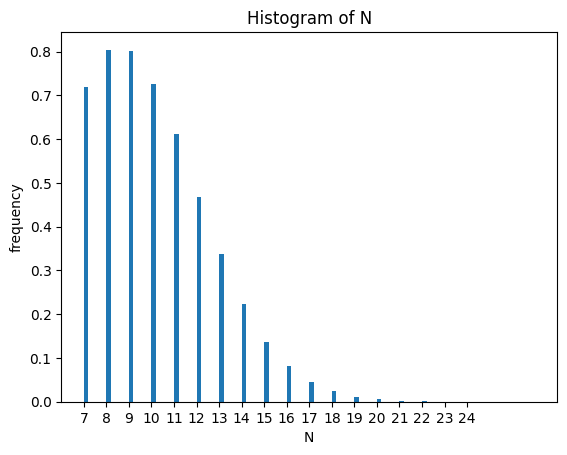
\includegraphics[width=0.49\textwidth]{./figure/p8/Gibbs_N.png}
\end{figure}

The estimated P given $X = 7$ has mean: $0.68449$, variance: $0.03196$.

(b) Directly calculate the posterior distribution of $P$ with Metropolis-Hastings algorithm:
\begin{align*}
f_{P|X}(p|X=x) &\propto P(X=x|P=p)f_P(p) \\
&= e^{-(\lambda p)}\dfrac{(\lambda p)^x}{x!} \cdot \dfrac{1}{\beta(a,b)}p^{a-1}(1-p)^{b-1} \\
&\propto e^{-\lambda p}(\lambda p)^x\cdot p^{a-1}(1-p)^{b-1}
\end{align*}
Since the support of $P$ is $[0,1]$, thus we can $\Unif(0,1)$ to be the proposal distribution, i.e. the one-step transition probability density from state $x$ to $y$ is $f_{i,j}=f_{X_{n+1}|X_n}(j|i)=1,j>0$, so we can get that the acceptance rate:
$$a_{i,j}=\min\left(\dfrac{\pi_jf_{j,i}}{\pi_if_{i,j}},1\right)=\min\left(\dfrac{e^{-\lambda j}(\lambda j)^x\cdot j^{a-1}(1-j)^{b-1}}{e^{-\lambda i}(\lambda i)^x\cdot i^{a-1}(1-i)^{b-1}},1\right)$$
The sampling results are as follows:
\begin{figure}[h]
    \centering
    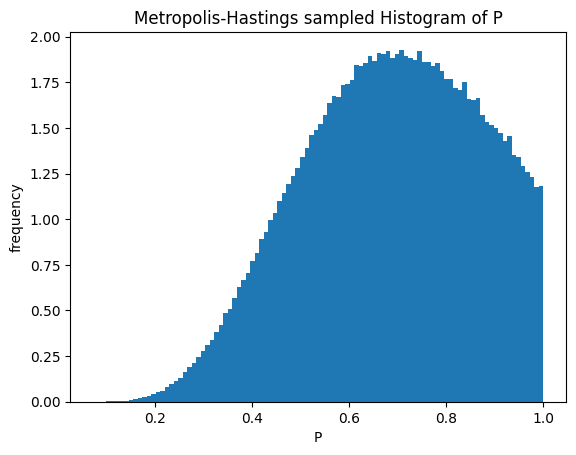
\includegraphics[width=0.6\textwidth]{./figure/p8/MH_P.png}
\end{figure}
The estimated P given $X = 7$ has mean: $0.68468$, variance: $0.03198$.

(c) We can see that both Gibbs sampling and Metropolis-Hastings algorithm with same sample number as burn in number have a similar estimation.

Metropolis-Hastings: \\
Advantages: It can sample many different distributions with suitable proposal distribution, without requiring the conditional distribution is easy to sample. \\
Disadvantages: It is actually a accept-reject method, if the simulation steps are not enough, it may reject many times and stay at the same state, also, it may need more calculations.


Gibbs sampling:
Advantages: It need less calculations, do not need to reject samples, thus it is efficient. \\
Disadvantages: It need to sample the conditional distribution, which required to be easy to sample. If the conditional distributions are complex, it still require Metropolis-Hastings algorithm or other sampling methods to generate a single sample, which is not efficient.

\end{homeworkProblem}

\newpage